\section{In-Plane Scour Scenarios}
\label{sec:dmem-scour-single-pier}

The first set of analyses considers longitudinal support loss, represented by $\eta_{s,x}$. Four single-pier scour locations are considered. The two intermediate piers are denoted as the left-bank pier (LBP) and the right-bank pier (RBP). For each pier, scour may develop on the overbank side (OBS) or on the channel side (CS). The four basic scenarios are therefore LBP-OBS, LBP-CS, RBP-OBS, and RBP-CS. Additional analyses combine support loss at more than one side or pier to investigate whether simultaneous scour effects are additive.

An initial screening analysis is performed using a longitudinal scour ratio of $\eta_{s,x}=0.17$ for the four single-pier locations. The objective is to identify which support-loss scenario most strongly affects the global load-carrying capacity.

\begin{figure}[htbp]
\centering
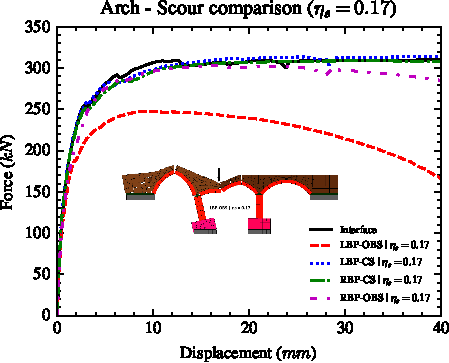
\includegraphics[width=0.82\linewidth]{./Figures/Arch_scour_comparison_1.pdf}
\caption{Influence of local longitudinal scour at different pier locations on the residual load-carrying capacity for $\eta_{s,x}=0.17$.}
\label{fig:dmem-scour-location-screening}
\end{figure}

The screening results in \Cref{fig:dmem-scour-location-screening} show that the response is strongly dependent on scour location. The critical scenario is scour on the overbank side of the left-bank pier (LBP-OBS), which produces a clear reduction in load capacity. By contrast, scour at the channel side of either pier has negligible influence for this geometry and loading configuration. This behaviour is governed by the direction of pier movement induced by the live-load mechanism. The bridge tends to mobilise pier rotation and displacement toward the overbank side; therefore, removing support from the side that is compressed and mobilised by the mechanism has a much larger effect than removing support from a side that progressively unloads.

\subsection{Left-Bank Pier Overbank-Side Scour}
\label{sec:dmem-scour-lbp-obs}

The LBP-OBS case is examined in more detail by increasing the longitudinal scour ratio. The capacity degradation curve is shown in \Cref{fig:dmem-scour-lbp-obs}.

\begin{figure}[htbp]
\centering
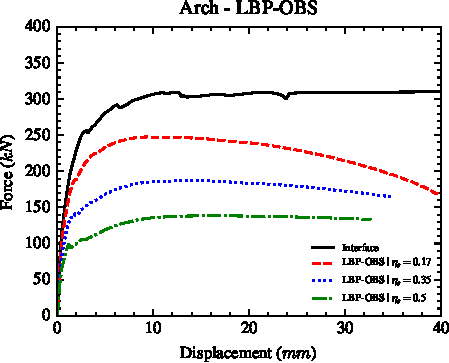
\includegraphics[width=0.82\linewidth]{./Figures/Arch_LBP_OBS.pdf}
\caption{Residual load-carrying capacity as a function of longitudinal scour ratio for overbank-side scour at the left-bank pier.}
\label{fig:dmem-scour-lbp-obs}
\end{figure}

The results show a progressive reduction in residual capacity with increasing $\eta_{s,x}$. This confirms that the left-bank pier is the controlling support for the considered load position and bridge geometry. Mechanistically, the loss of support modifies the rotation pattern of the pier and reduces the ability of the foundation interface to provide stabilising reaction. As the support loss increases, the arch-pier system reaches the collapse mechanism at lower live-load levels.

\subsection{Right-Bank Pier Overbank-Side Scour}
\label{sec:dmem-scour-rbp-obs}

The overbank side of the right-bank pier is also investigated because the no-scour pier displacement response suggests that this side may become relevant as the mechanism develops.

\begin{figure}[htbp]
\centering
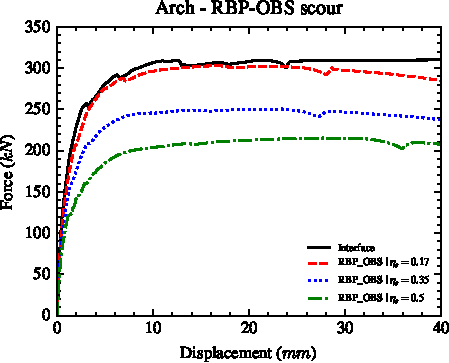
\includegraphics[width=0.82\linewidth]{./Figures/Arch_RBP_OBS.pdf}
\caption{Residual load-carrying capacity as a function of longitudinal scour ratio for overbank-side scour at the right-bank pier.}
\label{fig:dmem-scour-rbp-obs}
\end{figure}

For the initial scour ratio $\eta_{s,x}=0.17$, the RBP-OBS case does not significantly reduce the bridge capacity. At larger scour ratios, a gradual decrease becomes visible, but the degradation rate remains lower than for the LBP-OBS scenario. This indicates that the bridge mechanism mobilises the right-bank pier less critically for the selected load position, so support loss at that location is less damaging unless the erosion becomes severe.

\subsection{Uniform Scour at the Left-Bank Pier}
\label{sec:dmem-scour-lbp-uniform}

Additional analyses extend scour at the left-bank pier from the overbank side to the channel side, representing a more uniform loss of support below the same foundation.

\begin{figure}[htbp]
\centering
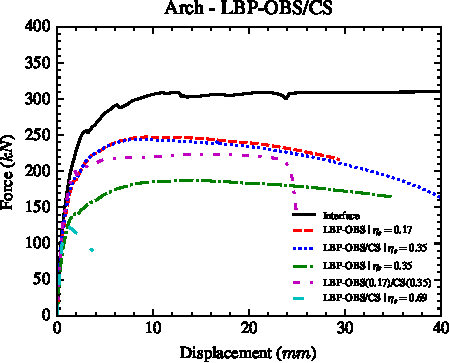
\includegraphics[width=0.82\linewidth]{./Figures/Arch_LBP_OBS_CS.pdf}
\caption{Residual load-carrying capacity for combined overbank-side and channel-side scour at the left-bank pier.}
\label{fig:dmem-scour-lbp-uniform}
\end{figure}

Adding channel-side scour to an existing LBP-OBS scenario does not necessarily cause an additional reduction in capacity. This response is explained by the pier kinematics. During rotation, the channel-side portion of the foundation progressively unloads and may partially detach from the supporting soil. Removing support from an already unloading region has little influence on the global collapse load. However, when the total uniform support loss becomes very large, the governing mechanism changes. Instead of being controlled primarily by pier rotation, the response becomes controlled by the bearing capacity of the remaining soil support.

\section{Combined Pier Scour}
\label{sec:dmem-scour-combined}

The final set of analyses considers simultaneous scour at both piers. These scenarios are relevant because real flood events may erode several foundations at the same time, even if the severity and side of erosion differ between piers.

\begin{figure}[htbp]
\centering
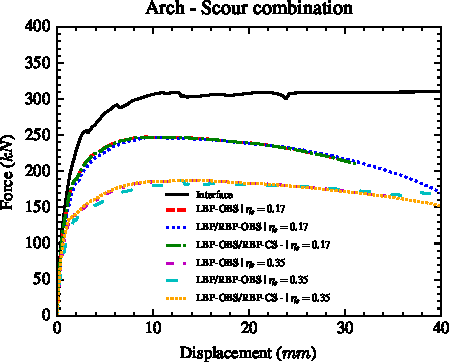
\includegraphics[width=0.82\linewidth]{./Figures/Arch_scour_combination.pdf}
\caption{Residual load-carrying capacity under combined scour scenarios involving both piers.}
\label{fig:dmem-scour-combined}
\end{figure}

\Cref{fig:dmem-scour-combined} shows that the response remains governed by the LBP-OBS scenario. Introducing additional scour at the right-bank pier does not further reduce the load capacity beyond that caused by the critical left-bank support loss. The collapse mechanism localises at the left-bank pier and develops before significant mobilisation of the opposite pier occurs. For this bridge and loading arrangement, the effect of simultaneous scour is therefore not additive.

This result is important for risk modelling. It suggests that the criticality of scour scenarios cannot be inferred only from the total amount of eroded support. The location of support loss relative to the bridge mechanism may be more important than the overall eroded area. Consequently, fragility models based on scour intensity should account for where scour occurs and how it interacts with the structural load path.

\section{Implications of the In-Plane Results}
\label{sec:dmem-scour-framework}

The in-plane analyses provide the first direct connection between the validated \gls{DMEM} model and the flood-risk theme of the thesis. The results indicate that residual load-carrying capacity can be expressed as a function of a support-loss parameter, $\eta_{s,x}$, and that this function depends strongly on the location of scour and on the governing in-plane mechanism. This type of response model can later be used to define engineering demand parameters, damage states, fragility functions, and performance indicators for risk and resilience assessment.

The analyses also show that computational efficiency is essential. Each nonlinear analysis can be completed within minutes on standard hardware, making repeated scenario analyses feasible. This is a necessary condition for future sensitivity studies, uncertainty propagation, and screening of bridge portfolios. The model is not yet a complete risk framework, but it provides the structural-analysis component required to translate flood-induced support degradation into residual capacity and failure mechanisms.
